\documentclass[sigconf]{acmart}

\usepackage{hyperref}

%\usepackage{endfloat}
%\renewcommand{\efloatseparator}{\mbox{}} % no new page between figures

\usepackage{booktabs} % For formal tables

\settopmatter{printacmref=false} % Removes citation information below abstract
\renewcommand\footnotetextcopyrightpermission[1]{} % removes footnote with conference information in first column
\pagestyle{plain} % removes running headers




\begin{document}
	\title {A comparative study of Kubernetes and Docker Swarm and Advantages of Singularity Container to HPC World}
	
	
	\author{Anand Sriramulu}
	\orcid{1234-5678-9012}
	\affiliation{%
		\institution{Indiana University}
		\streetaddress{107 S Indiana Ave}
		\city{Bloomington} 
		\state{Indiana}
		\country{USA}
		\postcode{47405}
	}
	\email{asriram@iu.edu}
	
	
	% The default list of authors is too long for headers}
	\renewcommand{\shortauthors}{Anand S}
	
	
	\begin{abstract}
		To discuss on the Container orchestration and comparing the most popular orchestrations Docker Swarm and Kubernetes on the areas of provisioning, configuration, discovery, monitoring, administration, rollback and placement policies. Providing high level overview on the advantages of the Singularity Containers over the others and how it benefits HPC workloads.
	\end{abstract}
	
	\keywords{i523, hid338, Docker Swarm, Kubernetes, Singularity}
	
	\maketitle
	
	\section{Introduction}
	Technology professional see the advantage of using a microservices architecture, wherein the application comprises of loosely coupled
	components, such as load balancers, caching proxies, message brokers, web servers, application services, and databases.
	The use of microservices allows developers to quickly create applications. In addition, this architecture saves a tremendous
	amount of resources in scaling applications, since each component can be scaled separately.
	Containers make it easy to deploy and run applications using the microservices architecture. They are lighter-weight compared
	to VMs and make more efficient use of the underlying infrastructure. Containers are meant to make it easy to scale applications,
	meet fluctuating demands, and move apps seamlessly between different environments or clouds. 
	Container orchestration tools can provide placement, scheduling, deployment, updates, health monitoring, scaling and failover functionality. 
	\cite{Container-Orchestration}	
	\section{Container Orchestration Functions }
	Here are some of the capabilities that a modern container orchestration platform will typically provide:
	\subsection{Provisioning}
	Container orchestration tools deals with provisioning or scheduling containers within the cluster and launching them.
	This process involves determining the appropriate host for the placement of the containers based on different constraints like
	resource requirements, location afinity, etc. The underlying goal is to increase utilization of the available resources.
	Apart from a container-provisioning API, orchestration tools will invoke the infrastructure APIs specific to the host 
	environment. \cite{Provisioning}
	\subsection{Declarative Configuration}
	Container orchestration tools provide options for the DevOps team to define the blueprint for an application workloadand its
	configuration in a standard schema using languages like YAML or JSON. The definitions includes informations related to repositories,
	networking, storage and logs to support the workload. Defining the blueprint in this manner makes it easy for DevOps teams to edit, 
	share and version the configurations and provide repeatable	deployments across development, testing and production.  \cite{Configuration-as-text}
	\subsection{Service Discovery}
	Container discovery becomes critical as the containers are running on multiple hosts in a distributed deployment environment.
	Web servers need to dynamically discover the web servers and the load balancers need to discover and register the web servers.
	Orchestration tools uses a distributed  key-value based  store as lightweight DNS mechanism to discover the containers.
	\subsection{Monitoring}
	Container orchestration tools are aware of the configuration to track and monitor the health of the containers and hosts in the cluster. 
	If a container crashes, a new one can be spun up quickly. If a host fails, the tool can relocate the failed containers on another host.
	It will also run specified health checks at the appropriate frequency and update the list of available nodes based on the results. The tool will 
	ensure that the deployment matches the desired state of the cluster matches the configuration specified. 
	\subsection{Rolling Upgrades and Rollback }
	Some orchestration tools can perform 'rolling upgrades' of the application where a new version is applied incrementally
	across the cluster. Traffic is routed appropriately as containers go down temporarily to receive the update. A rolling update
	guarantees a minimum number of "ready" containers at any point, so that all old containers are not replaced if there aren't
	enough healthy new containers to replace them. If, however, the new version doesn't perform as expected then the
	orchestration tool may also be able to rollback the applied change. 
	\subsection{Policies for Placement, Scalability etc.}	
	Container orchestration tools provide a way to define policies for host placement, security, performance and high availability.
	When configured correctly, container orchestration platforms can enable organizations to deploy and operate containerized
	application workloads in a secure, reliable and scalable way. For example, an application can be scaled up automatically based
	on CPU usage of the containers. 
	\subsection{Administration}	
	Container orchestration tools should provide mechanisms for administrators to deploy, configure and setup. An extensible
	architecture will connect to external systems such as local or cloud storage, networking systems etc. They should connect to
	existing IT tools for SSO, RBAC etc. 
	
	\section{Kubernetes}
	Kubernetes is a Goolge product and they used it for their running their heavy workloads in production.	
	Kubernetes website says, "Kubernetes is an open-source system for automating deployment, scaling, and management of containerized applications."
	It an architecture based on master server and multiple nodes(minions). To manage and orchestrate the nodes, kubecfg (Command line tool) is
	used to connects to the API endpoint.
	Definitions of the components within the Kubernetes environment:\newline
	\textbf{Master:} The server that runs the Kubernetes processes like API service, scheduler and replication controler.\newline
	\textbf{Node:} The hosts that runs the kubelet service and the containers engine. The node receives command from the Master.\newline
	\textbf{Kubelet:} It's a node lever manager.\newline
	\textbf{Pod:} Collection of containers deployed to the same node.\newline
	\textbf{Replication Controller:} Defines the number of pods or containers need to be running.\newline
	\textbf{kubecfg:} Command line interface to manage the kubernetes deployment. \newline
	\cite{Kubernetes}
	\begin{figure}[h]
		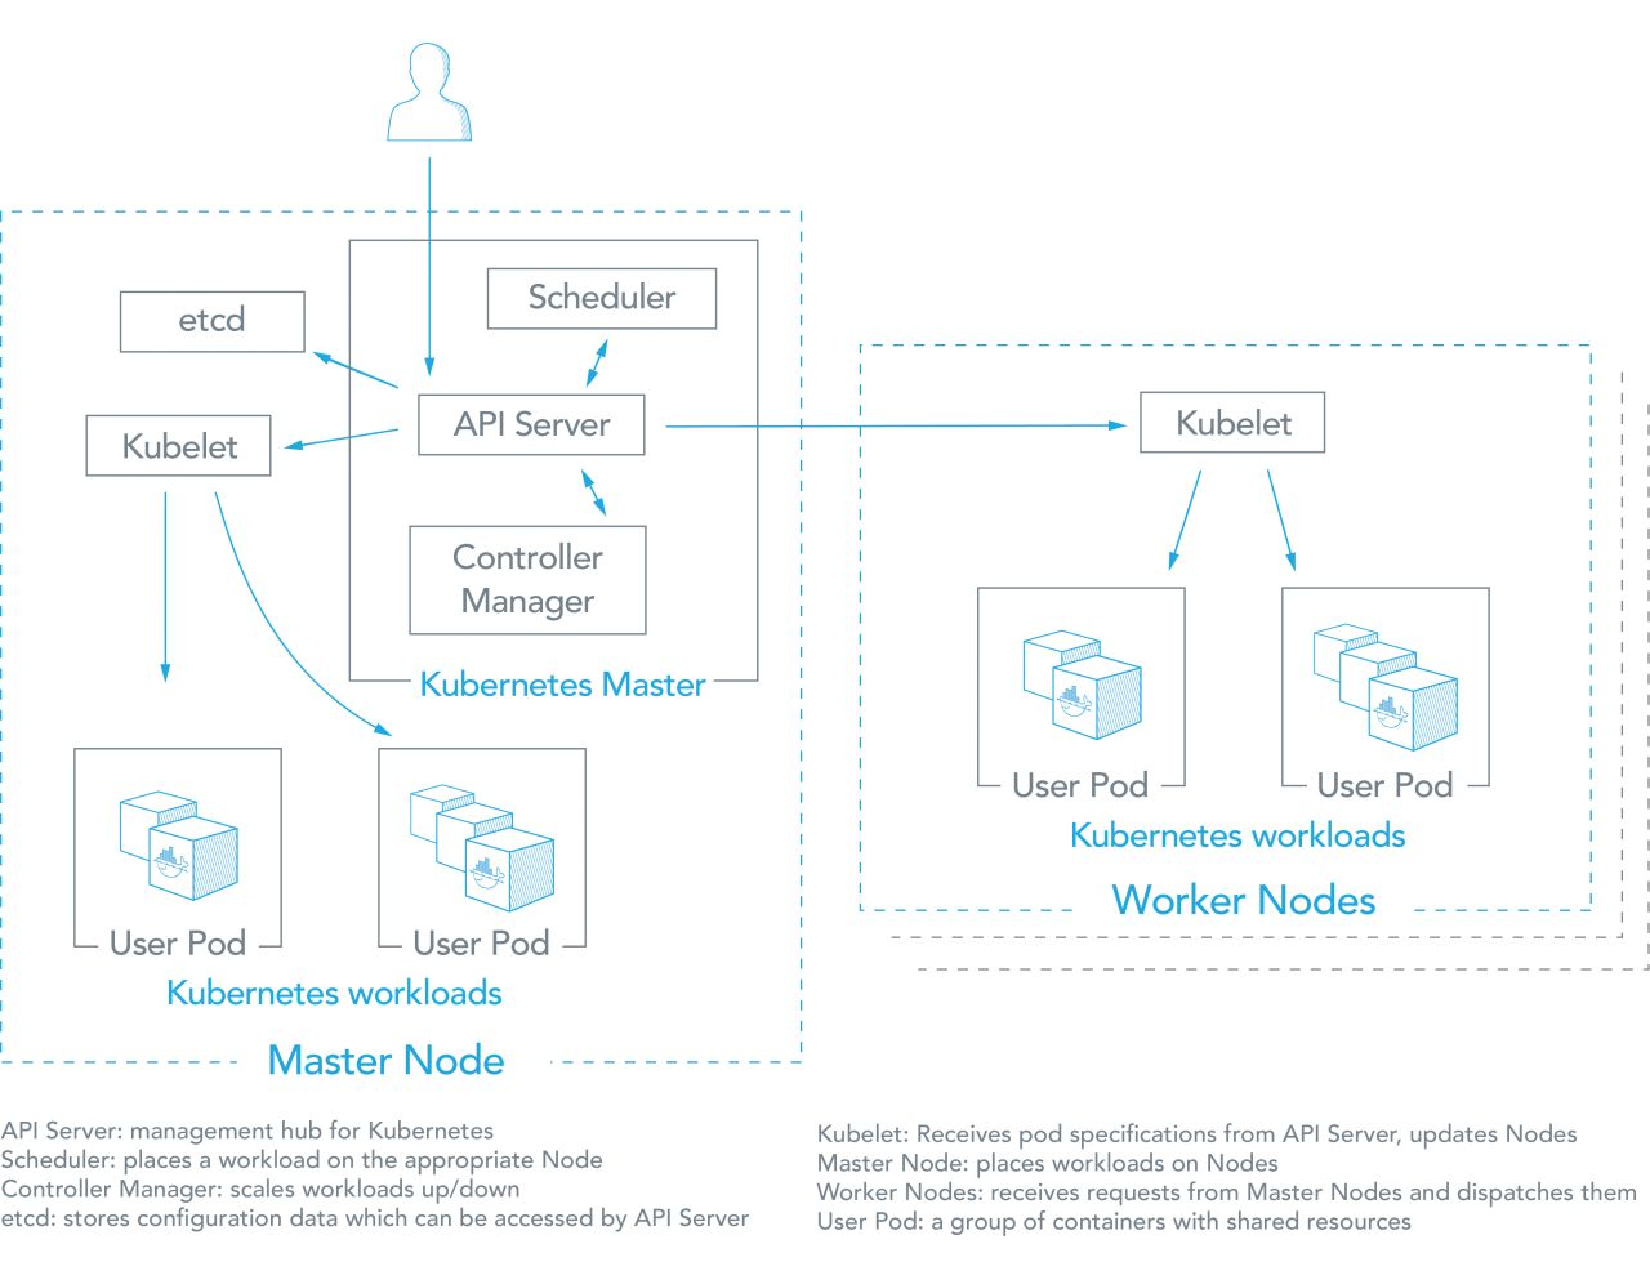
\includegraphics[width=0.5\textwidth]{images/Kubernetes}
		\caption{Kubernetes Nodes Illustration \cite{Platform9}.} \label{fig:figure1} 
	\end{figure}
	
	\section{Docker Swarm}
	Docker swarm is a simple container orchestrion and yet it's powerful. It uses the same Docker API with the core Docker engine. The swarm manages pool of 
	Docker engines with an endpoint in which it benefits the existing tools and APIs as it work with the cluster the same way it work with a docker instance.
	The Docker Swarm has in-built scheduling strategies as the containers can be placed across the cluster and also it supports random placement.
	Swarm uses a pluggable back-end architecture that works with a simple hosted discovery service, static files, etcd, Zookeeper, Consul,lists of IPs.
	
	\begin{figure}[h]
		\includegraphics[width=0.5\textwidth]{images/DockerSwarm}
		\caption{Docker Swarm Architecture \cite{Platform9}.} \label{fig:figure2} 
	\end{figure}
	
	\section{Kubernetes vs Docker Swarm}
	Both the contrainer orchestration offers similar functionalities, but I will discuss on the pros and cons here.
	\cite{kubernetes-vs-docker-swarm}
	\subsection{Application definition}
	Kubernetes can be deployed in combination of pods and micro-services. Docker, whereas applications can be deployed as micro-services.
	\subsection{Installation and Setup}
	
	Kubernetes is not very easy in terms of setup, but Google provides good documentation for the setup. It takes lot of time for the developer to get the setup done.
	On the other hand, Docker Swarm doesn't need much learning for the developers or devops and has easy process to setup and manage with the help of Command Line Interface (CLI).
	Overall, Docker wins here.
	
	\subsection{Monitoring and Logging}
	Both Kubernetes and Docker Swarm doesnt provide inbuilt support but extent offers logging and monitoring thru third party libraries. 
	With Docker, DataDog, Reimann, Retrace and Sumo Logic can be used.
	With Kubernetes, Kibana and ElasticSearch can be used for Logging and Influx, Grafana, Heapster for Monitoring.
	
	\subsection{Size and Performance}
	Both can support 1000 node clusters in which each cluster can support up to 30,000 containers.
	\subsection{Conclusion}
	The best way to decide between the tools is probably to consider which one is more familiar and suits the existing software stack. 
	Docker Swarm is a simple and easy solution to work with whereas Kubernetes is targeted those who requires support for complex applications.
	\section {Singularity Container and Features}
	As per Singularity website "Singularity containers can be used to package entire scientific workflows, software and libraries, and even data. This means that you don't have to ask your cluster admin to install anything for you - you can put it in a Singularity container and run"
	
	\begin{figure}[h]
		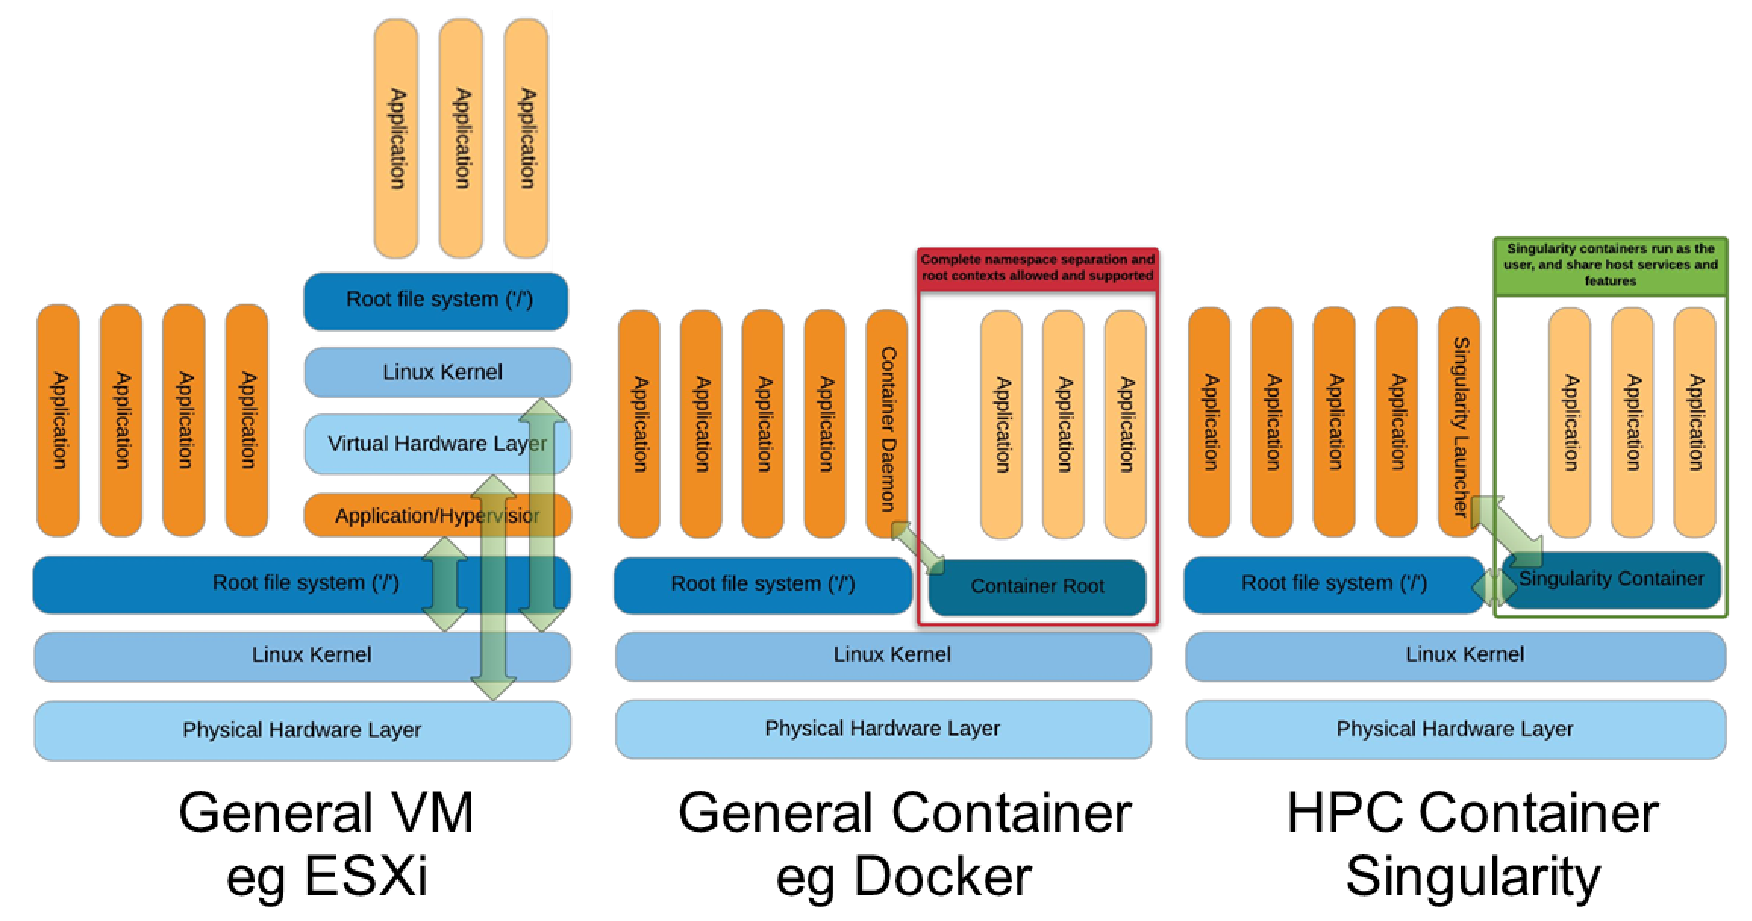
\includegraphics[width=0.5\textwidth]{images/vm_docker_singularity}
		\caption{VM vs Docker vs Singularity \cite{vmDockerSingularity}.} \label{fig:figure3} 
	\end{figure}
	
	Singularity containers is different from other containers due to the following aspects:
	\textbf{Application Portability} - Single Image File which contain all dependencies. Reproducibility, run cross platform and support legacy operating system and applications.\newline
	\textbf{Docker Integration} - It can convert Docker images into Singularity images easily \newline
	\textbf{User Group Focus} - It focuses on Scientific Application Users \newline
	\textbf{Filesystem} - Docker has no direct access to the host's filesystem except the directories are available cross mounted in the container. But for scientific computing, the access to host's files, data and libraries is needed. With Singularity process that is running as the user see the user's home directory and hence the user's environment is shared. \newline
	\textbf{Security Model} - It's the key aspect that it can be used with unprivileged permissions and doesn't require a separate daemon process. In which it highly useful in HPC workloads.\newline
	Docker containers run with root privileges in the container's operating system, which is not a problem if the container is running on a VM. But
	it's a security risk, if the container is running on a shared environment like university or super computer lab as the user can access the
	Docker daemon with the root access. Singularity solves the issue with creating and running the container with the user identity, so the permissions for the user will be same for both inside and outside the container.\newline
	\cite{Singularity}
	
	\begin{acks}		
	
	The author would like to thank Dr. Gregor von Laszewski and the Teaching Assistants for their support and valuable suggestions.
	
	\end{acks}
	\bibliographystyle{ACM-Reference-Format}
	\bibliography{report} 
	
\end{document}
